\chapter{Introducere}

\section{Context}

Este dovedit faptul că \textit{educația avansată} reprezintă motorul principal al progresului ce stă la baza obiectivelor de dezvoltare durabilă la nivel global. \textit{Educația terțiară} este percepută ca fiind catalistul pentru dezvoltare și sustenabilitate \cite{educationParticipantsOECD}. Așadar, se poate aprecia faptul că este imperios pentru societate să formeze cât mai multe persoane cu studii superioare absolvite în vederea atingerii dezvoltării și prosperității viitoarelor generații.

\begin{figure}[H]
    \centering
    \textbf{Tendințe în ponderile tinerilor cu vârste cuprinse între 25-34 de ani cu studii superioare (în perioada 2000 – 2021)}\par\medskip
    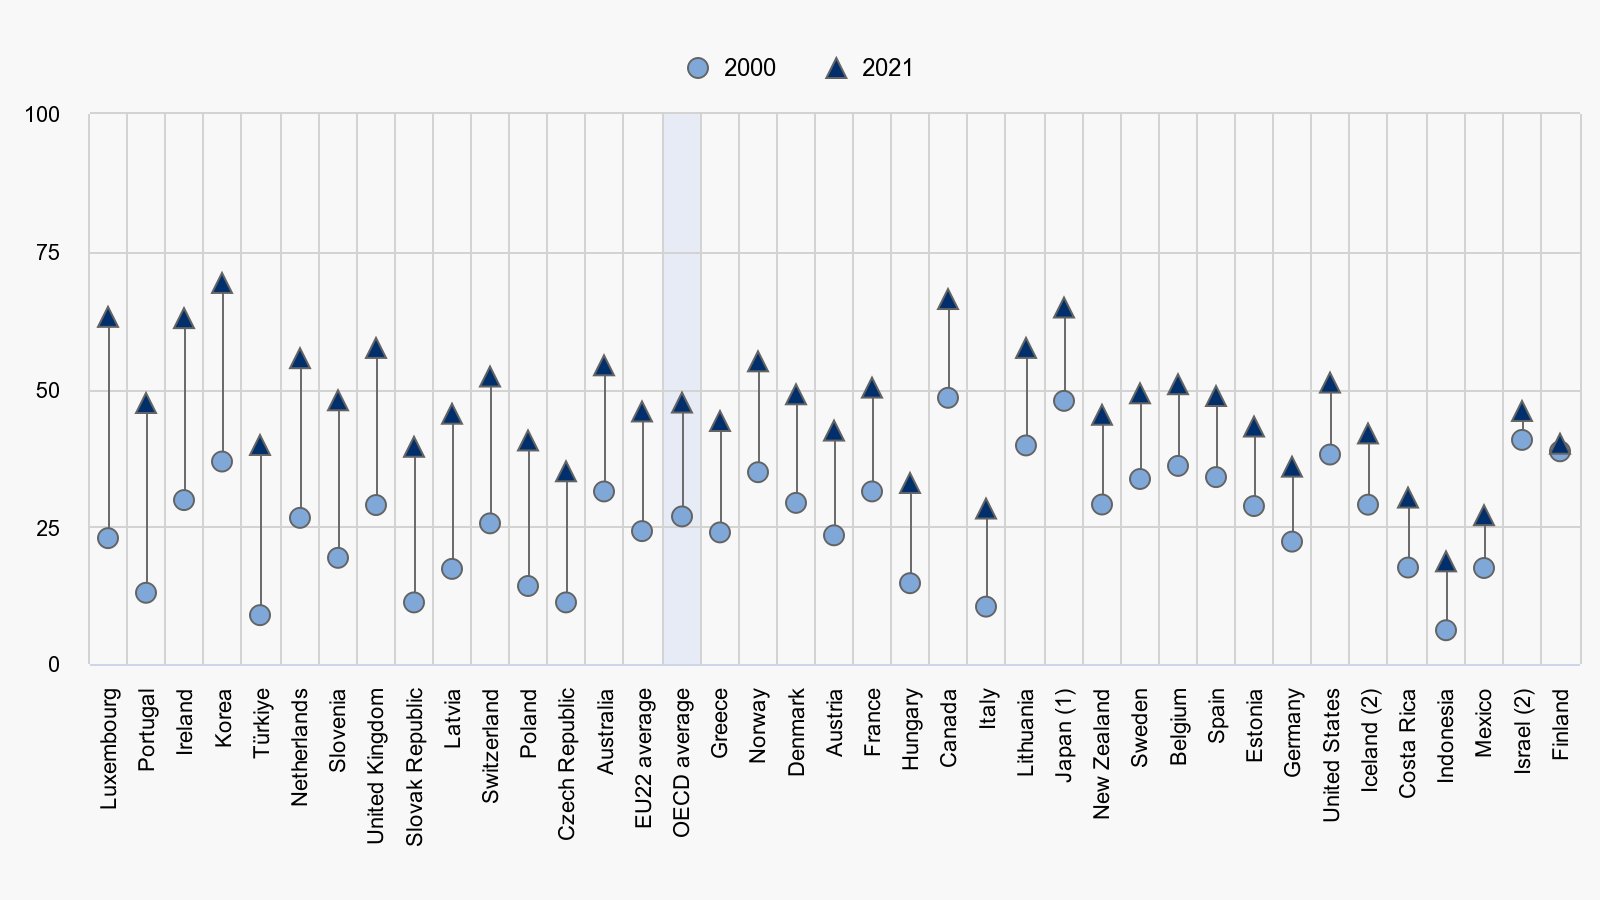
\includegraphics[width=.9\linewidth]{trends-tertiary-educated-adults.png}
    \caption{Țările sunt ordonate în funție de diferența procentuală de persoane cu studii superioare între anii 2000-2021. Datele includ și programele superioare după licență și cele post-secundare non-terțiare \cite{levelAdultsStudiedOECD}}
\end{figure}

Datorită condițiilor globale de natură economico-politică, înscrierile la școli au crescut, favorizate și de obligativitatea școlară la nivel de bază. Numărul persoanelor cu vârste cuprinse între 25 și 34 de ani ce au decis să urmeze un program de studii superioare s-a mărit foarte mult în majoritatea țărilor din OECD. Ponderea medie a tinerilor adulți care au studii superioare aproape s-a dublat în perioada 2000-2021 (de la aproximativ 27\% în 2000 la 48\% în 2021). Dacă trendul curent al educației digitalizate continuă să se dezvolte, se consideră că educația superioară va fi cea mai comună realizare printre adulții din spațiul muncii în următorii ani \cite{levelAdultsStudiedOECD}.

Pentru a încuraja și a ajuta tinerii în atingerea țelului de a obține o educație superioară, societatea a creat diferite materiale și produse care să vină în sprijinul studenților și a le facilita procesul de învățare continuă (de la cărți la materiale video, și diverse aplicații).

Printre numeroasele metode pe care le folosesc studenții și elevii în vederea eficientizării procesului de învățare se numără \textit{flashcard-urile}. Această metodă de învățare este populară atât în rândul studenților care trebuie să memoreze cât mai multe informații (precum cei de la medicină sau drept), cât și al elevilor care învață o nouă limbă străină. Studenții de la medicină sunt nevoiți să învețe un volum foarte mare de informații într-un timp cât mai scurt, motiv pentru care se folosesc de flashcard-uri pentru a fi cât mai eficienți posibil și a stoca informațiile în memoria de lungă durată \cite{in2med}.

Flashcard-urile pot varia de la a fi \textit{foarte simple} (caz în care cele mai importante cuvinte sunt colorate diferit) la a fi \textit{foarte complexe} (unde pot conține poze sau desene). S-a observat faptul că utilizarea culorilor cu scopul de a coda, a memora și a reîmprospăta informația reținută în memorie permite o creștere semnificativă a ratei de învățare, în special în rândul adulților \cite{journalEducation}.

\noindent\begin{minipage}{0.6\textwidth}
    \begin{figure}[H]
    \centering
    \textbf{Exemple de cartonașe pentru medicină}\par\medskip
    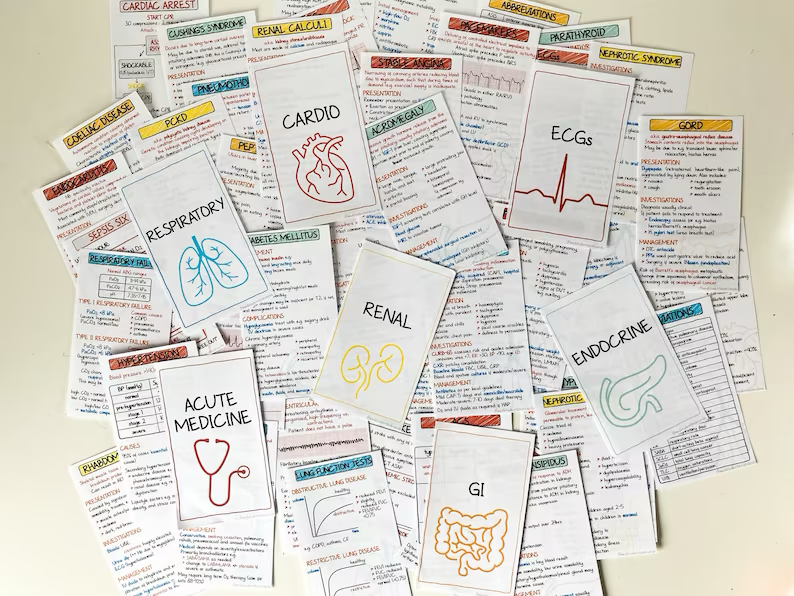
\includegraphics[width=\linewidth]{cartoanse-medicina-etsy.png}
    \caption{Diverse exemple de cartonașe pentru domeniul medicinii, folosindu-se de diferite desene, grafice și culori \cite{etsyPaperFlashCardsMedicine}} 
    \label{fig:cartonase}
    \end{figure}
\end{minipage}
\hfill
\begin{minipage}{0.35\textwidth}
    Înainte de era digitalizării, studenții foloseau flashcard-uri din hârtie (câteva exemple pot fi vizualizate în figura \ref{fig:cartonase}). Acestea prezintă, de asemenea, dezavantaje, întrucât pot fi dificil de prezervat și de gestionat.

    În prezent, există diverse aplicații educative de tip flashcard ce oferă multiple beneficii și un management eficient al acestora. În cele ce urmează sunt prezentate patru astfel de aplicații.
\end{minipage}

\subsection{Aplicații similare}

\subsubsection{Ankie}

\noindent\begin{minipage}{0.6\textwidth}
    Proiectul \textit{Ankie} \cite{anki} este unul din cele mai populare și mai complexe aplicații de tip flashcard similare. Anki oferă suport pentru imagini, audio, video și text științific pentru flashcard-uri. Printre principalele caracteristici se pot enumera: sincronizarea între dispozitive, aplicații pentru cele trei sisteme de operare pe desktop și laptop (Windows, Mac, Linux), dar și pentru mobil (Android și iOS). Proiectul este complet open source și are ca main selling feature faptul că este customizabil prin crearea de plugin-uri. Singura problemă menționată de utilizatori este aceea că aplicația este foarte complexă, ceea ce produce dificultăți persoanelor noi care tocmai au accesat aplicația.
\end{minipage} 
\hfill
\begin{minipage}{0.35\textwidth}
    \begin{figure}[H]
    \centering
    \textbf{Aplicația Ankie}\par\medskip
    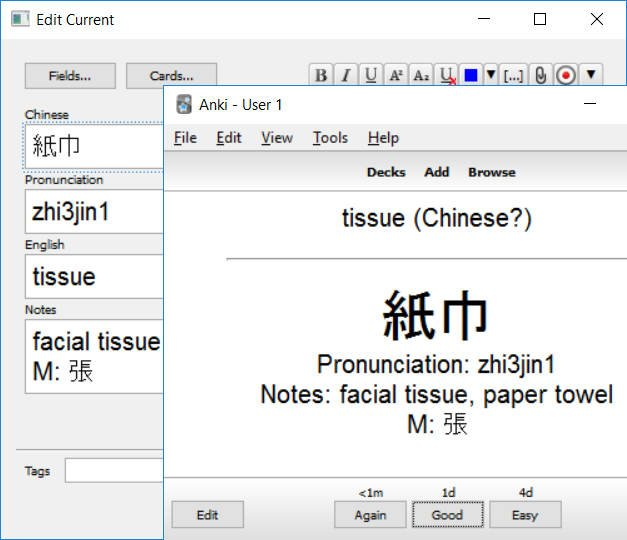
\includegraphics[width=\linewidth]{ankie.jpg}
    \caption{Exemplu de creare a unui cartonaș pentru o limbă străină \cite{ankiImageExample}} 
    \label{fig:exemplu_ankie}
    \end{figure}
\end{minipage}

\bigbreak
Caracterul de complexitate prezintă avantajul de a folosi proiectul Ankie în mai multe scopuri, precum învățarea unei noi limbi străine ori pregătirea pentru examene de medicină sau de drept. Alt avantaj ar fi faptul că nu este nevoie de un cont pentru a putea utiliza principalele caracteristici ale aplicației (excepție făcând sincronizarea cartonașelor între dispozitive).

\subsubsection{Memrise}

\noindent\begin{minipage}{0.35\textwidth}
    \begin{figure}[H]
        \centering
        \textbf{Aplicația Memrise}\par\medskip
        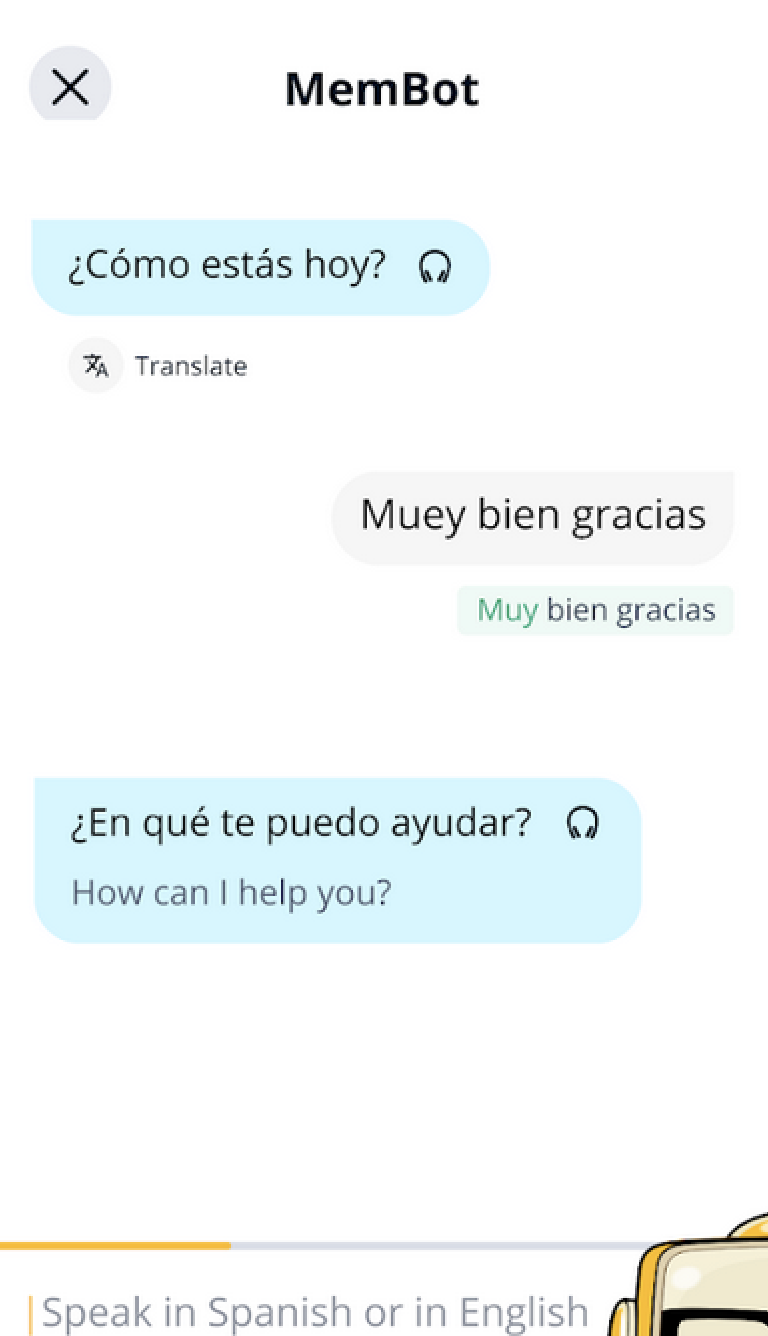
\includegraphics[width=.8\linewidth]{memrise.png}
        \caption{Exemplu de conversație în aplicația Memrise \cite{memriseImageExample}} 
        \label{fig:exemplu_memrise}
    \end{figure}
\end{minipage} 
\hfill
\begin{minipage}{0.55\textwidth}
   Aplicatia \textit{Memrise} \cite{memrise} este disponbilă doar pentru dispozitivele mobile. Principalul selling factor este de a învăța o nouă limbă străină. Proiectul oferă cursuri pentru 23 de limbi, ofera quizuri, videoclipuri cu traduceri de către vorbitori nativi. Un nou feature adus de această aplicație este practicarea vorbitului unei noi limbi folosind GPT-3, drept partener AI de conversație (exemplu în figura \ref{fig:exemplu_memrise}. Aplicația oferă atât un plan free cât și unul plătit și este de tip proprietar. Dezavantajul aplicației constă în faptul ca targetează doar învățarea limbilor străine, deși excelează în acest domeniu oferind cursuri.
\end{minipage}

\subsubsection{Quizlet}

\noindent\begin{minipage}{0.55\textwidth}
    Aplicatia \textit{Quizlet} \cite{quizlet} reprezintă un alt competitor, bazându-se pe acoperirea mai multor domenii, printre care se numără: examene, arte, limbi străine și științe. De asemenea, aceasta are un market pentru folosirea altor seturi de cartonașe pentru învățare. Anumite seturi de cartonașe „curated”, aparținând creatorilor aplicației, denotă unul dintre avantajele aplicației. Quizlet oferă atât un plan gratuit, cât și unul plătit, fiind de tip proprietar, ca în cazul aplicației Memrise. Dezavantajul aplicației Quizlet este reprezentat de faptul că planul gratuit are forma unui demo, ba mai mult, este destul de limitat în atragerea utilizatorilor. Un alt dezavantaj este acela că, fiind o aplicație proprietară, nu pot fi adăugate plugin-uri sau extensii.
\end{minipage} 
\hfill
\begin{minipage}{0.35\textwidth}
    \begin{figure}[H]
        \centering
        \textbf{Aplicația Quizlet}\par\medskip
        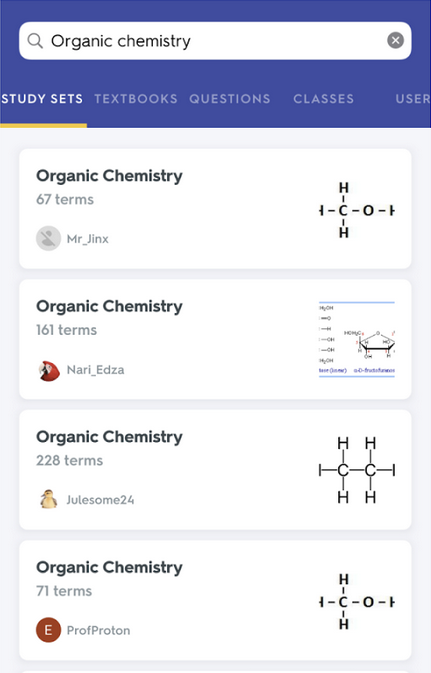
\includegraphics[width=\linewidth]{quizlet.png}
        \caption{Exemplu de pachete în aplicația Quizlet \cite{quizletImageExample}} 
        \label{fig:exemplu_quizlet}
    \end{figure}
\end{minipage}

\subsubsection{Brainscape}

\noindent\begin{minipage}{0.35\textwidth}
    \begin{figure}[H]
        \centering
        \textbf{Aplicația Brainscape}\par\medskip
        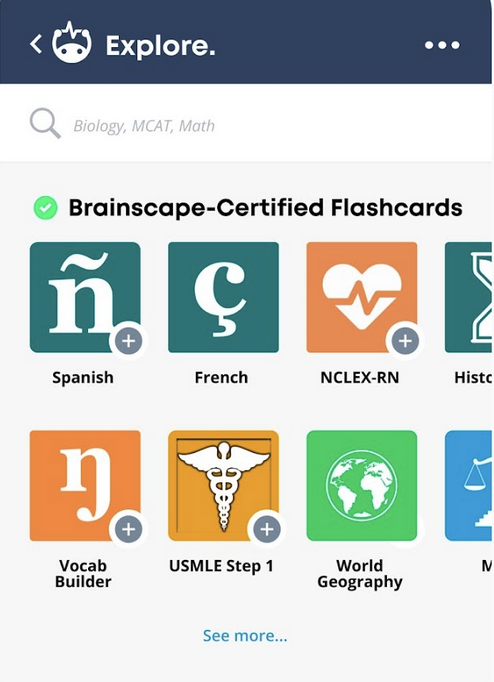
\includegraphics[width=\linewidth]{brainscape.png}
        \caption{Exemplu de pachete în aplicația Brainscape \cite{brainscapeImageExample}} 
        \label{fig:exemplu_brainscape}
    \end{figure}
\end{minipage} 
\hfill
\begin{minipage}{0.55\textwidth}
    Aplicația \textit{Brainscape} \cite{brainscape} reprezintă un alt competitor solid din acest segment. Principalii clienți ai aplicației activează în domeniul de business pentru training. Aceasta oferă suport pentru web și dispozitivele mobile, dar și planuri gratuite și plătite. Un avantaj ar consta în punerea la dispoziția utilizatorilor a unei game largi de cartonașe din varii domenii. Printre dezavantajele aplicației se numără suportul existent doar în versiunea de web, respectiv o aplicație proprietară fără suport pentru extensii.
\end{minipage}

\section{Scopul lucrării}

Scopul lucrării este acela de a crea o aplicație de mobil pentru principalele sisteme de operare (Android și iOS), orientată către studenții din STEM, care să le ofere un suport complementar în sistemul de învătare.

Aplicațiile prezentate în secțiunea anterioară au un public restrâns de utilizatori, motiv pentru care se urmărește ca noua aplicație creată să acopere o arie mai largă de nevoi. Astfel, aplicația \textit{Alfie} încurajează și crearea unor cartonașe de învățare pentru științele exacte, utilizările fiind, în principal, pentru ecuații și teoreme. Aplicația vine în ajutorul scrierii de text științific în cartonașe cu feature-ul de convertire a unei poze care conține text matematic în formatul TeX. Acesta ar fi un prim pas pentru studenții noi care nu ar cunoaște limbajul. Un convenient este reprezentat de faptul că orice utilizator are posibilitatea de a fotografia un text matematic (care poate să nu fie cel mai lizibil) și de a-l transforma într-un cartonaș lizibil. Pentru acest lucru aplicația se va folosi de un microserviciu cu rate limiter implementat. Microserviciul va primi imaginile de la utilizatori, le va comprima și le va trimite către api-ul de OCR oferit de Mathpix \cite{mathpixOCR}.

Aplicația \textit{Alfie} permite introducerea de cartonașe customizabile, astfel încât să acopere majoritatea usecase-urilor, propunând în acest sens cartonașe cu mai multe formatări pentru text (text fără formatare, HTML, Markdown cu suport pentru HTML și TeX). Motivul introducerii suportului pentru mai multe formatări este acela de a ușura tranziția în utilizarea aplicației. Pe lângă formatările de text, pot fi inserate imagini în fiecare cartonaș, atât pentru întrebare, cât și pentru răspuns. Implementarea conținutului vizual vine ca suport pentru învățarea prin imagini.

Un ultim lucru pe care și-l propune aplicația este să ofere suport de backup pentru cartonașe. Sistemul de backup este benefic pentru utilizatorii care își schimbă dispozitivul mobil din varii motive. În acest sens, aplicația Alfie implementează un dublu sistem de backup. Unul dintre sisteme este dedicat utilizatorilor fără cont, în care aplicația salvează conținutul media accesibil utilizatorului. De asemenea, se oferă suport pentru exportarea bazei de date a cartonașelor și importarea acesteia. Al doilea sistem de backup este unul în cloud folosind serviciul S3 de la AWS \cite{awsS3}. În cazul acestui sistem, utilizatorul trebuie să aibă un cont creat în aplicație. Sistemul de backup în cloud are avantajul că utilizatorii nu trebuie să își mai facă probleme în ceea ce privește backup-ul sau locul în care conținutul este salvat.

Aplicația are ca target ambele sisteme de operare majore pentru telefon (Android și iOS) și este dezvoltată folosind Flutter cu design Material pentru o interfață și experiență comună. Codul sursă pentru aplicația de mobil este public accesibil la adresa: \url{https://github.com/george-radu-cs/alfie-client}.

Pentru implementarea serviciilor de backup media, autentificare și ocr se vor folosi două microservicii. Așadar, în cazul autentificării utilizatorilor și al backup-ului media, se va apela la un server în Go, în timp ce pentru serviciul de ocr se va folosi un server în Node.js. Codul sursă pentru serviciile de cloud ale aplicației este public accesibil la adresa: \url{https://github.com/george-radu-cs/alfie-cloud-services}.

Un ultim scop al prezentei lucrări este acela de a demonstra într-un mod practic cunoștințele dobândite de către autor pe parcursul programului de licență, pe specializarea Informatică, cunoștințe din domenii diverse, precum: baze de date, structuri de date, algoritmi, tehnologii web \& mobile, rețele, protocoale de comunicații, securitate și dezvoltare software a produselor.

\section{Motivație}

Principala motivație ce stă la baza creării aplicației \textit{Alfie} este aceea de a dezvolta un produs calitativ care să fie util și eficient în procesul de învățare al altor studenți sau elevi. Prin feature-urile pe care le aduce aplicația în versiunea actuală, se dorește ușurarea procesului de învățare al studenților din STEM.

O altă motivație are un caracter mult mai personal și se bazează pe demonstrarea/ ilustrarea parcursului și a nivelului de cunoștințe dobândite în timpul facultății, respectiv a nivelului de adaptabilitate la noi încercări/tehnologii și dezvoltarea pe toate planurile profesionale. Printre acestea, se numără: servicii de backend, integrări cu api-uri 3rd party, clean code, design patterns, devops, dezvoltare mobile, înțelegerea clară a unei interfețe și crearea unei experiențe plăcute pentru utilizatorul final.
